\chapter{Tutorial 2: Simple Beam Model with MSML}

The medical simulation markup language (MSML) is a flexible XML-based description for the biomechanical modeling workflow and finite-element based biomechanical models.

The example files include several scenarios based on a simple beam model. One scenario describes a linear elastic beam under gravity load. If you are using the pre-built Docker container you can open the scenario with 
\begin{lstlisting}[language=sh, breaklines=true]
$ geany /opt/msml/examples/BeamExample/beamLinearGravity.msml.xml
\end{lstlisting}

In order to simulate the scenario the MSML exec command can be executed from the command line:
\begin{lstlisting}[language=sh, breaklines=true]
$ cd /opt/msml/src
\end{lstlisting}
\begin{lstlisting}[language=sh, breaklines=true]
$ ./msml.py exec -o outputfolderPath /opt/msml/examples/BeamExample/beamLinearGravity.msml.xml
\end{lstlisting}

To get the help information of MSML type the following:
\begin{lstlisting}[language=sh, breaklines=true]
$ ./msml.py -h (or for methods: $ ./msml.py exec -h)
\end{lstlisting}

ParaView can be used to view the results and inspect the meshes:
\begin{lstlisting}[language=sh, breaklines=true]
$ cd /opt/paraview/bin
\end{lstlisting}
\begin{lstlisting}[language=sh, breaklines=true]
$ ./paraview
\end{lstlisting}

After starting ParaView as shown in Fig. \ref{ParaViewScreenshot} you have to load the output file (
before you can press \emph{play} you have to click on \emph{Apply} in the tab \emph{Properties}). The output mesh for each timestep is usually labeled 'dispx.vtu'.

\begin{figure}[h]
  	\centering
    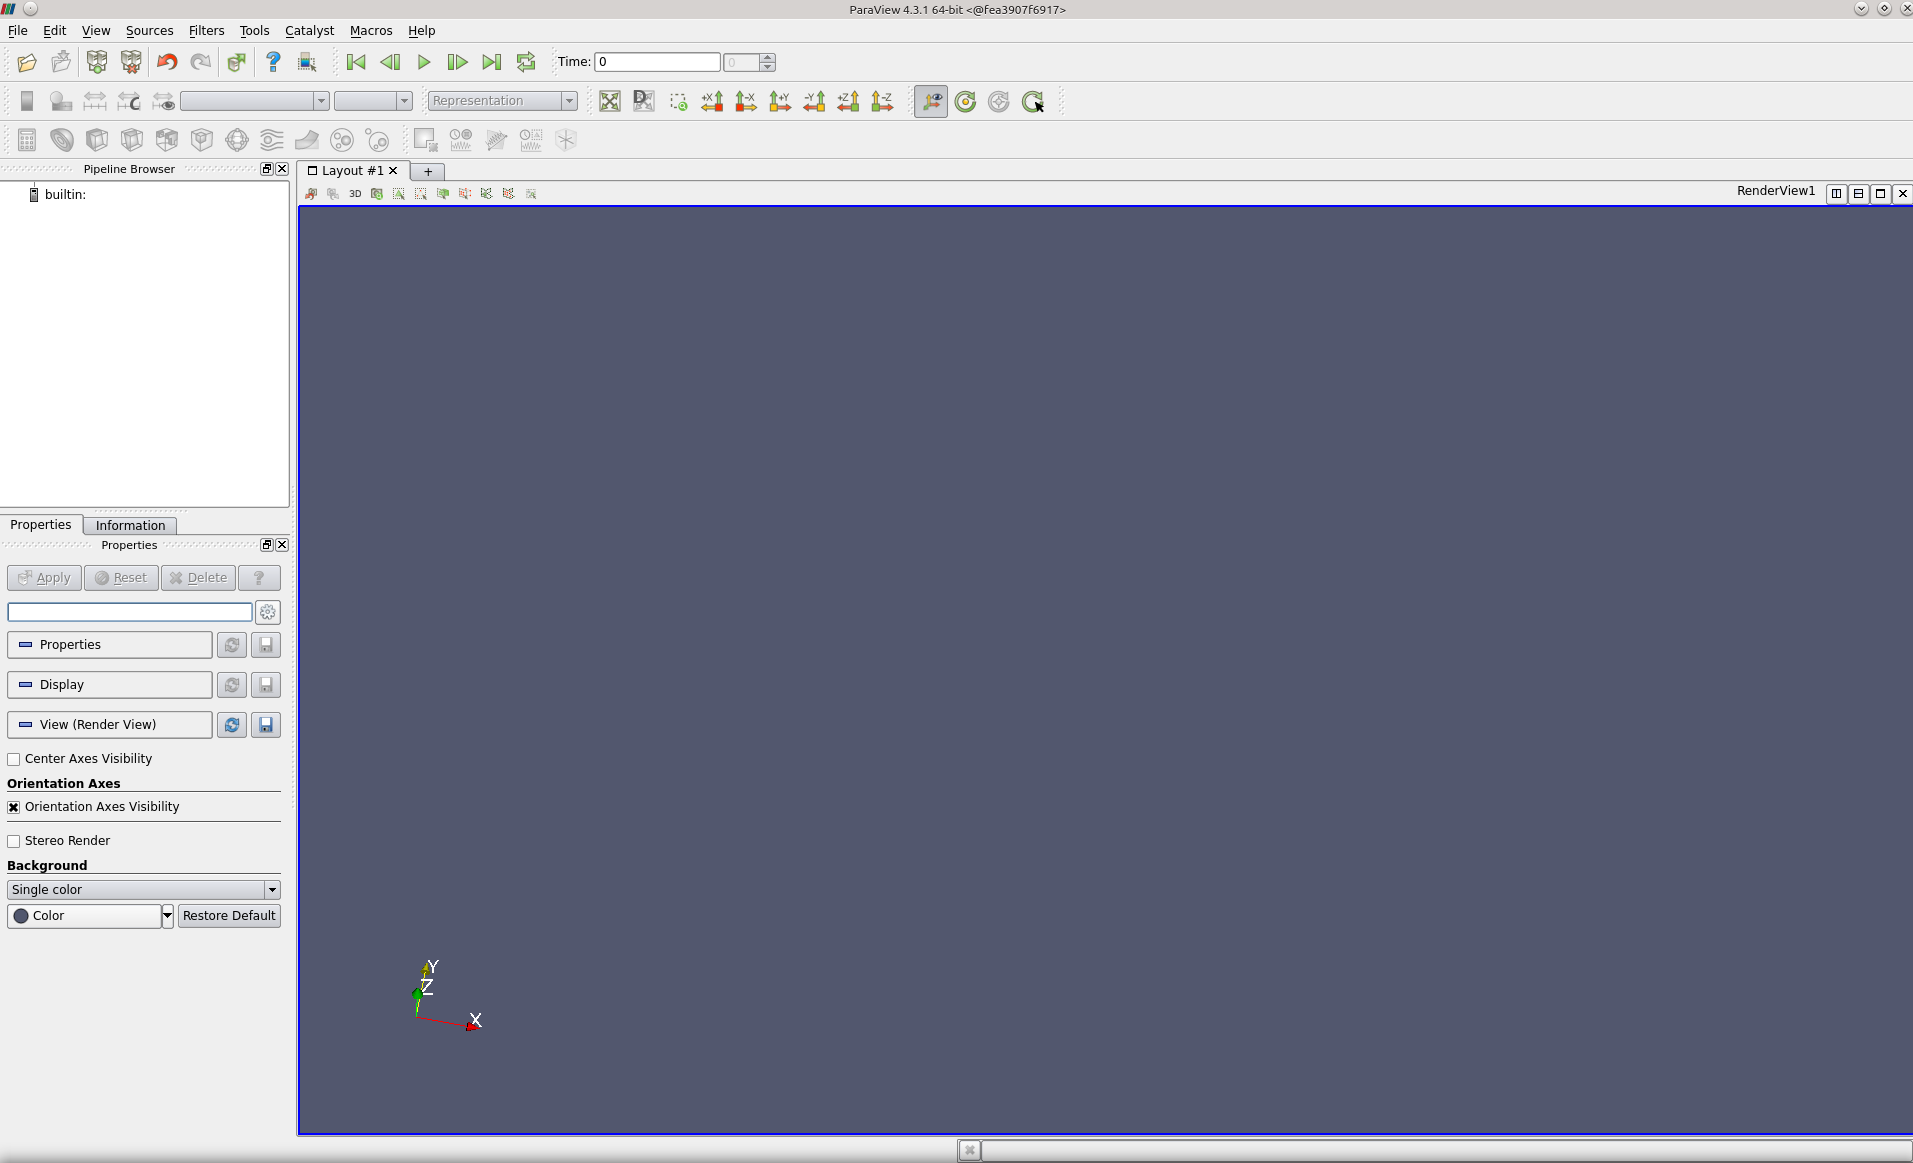
\includegraphics[width=\textwidth]{pictures/start_paraview.png}
    \caption{Start window of ParaView.}
    \label{ParaViewScreenshot}
\end{figure}

The scenario settings (e.g. material parameters, boundary conditions) can be changed by opening the XML-file in a suitable text editor, e.g.
\begin{lstlisting}[language=sh, breaklines=true]
$ geany /opt/msml/examples/BeamExample/beamLinearGravity.msml.xml &
\end{lstlisting}





\section{Using the Python API}

This section describes how to create a running script for MSML in Python.

First open an editor (e.g. geany) and create a new file \emph{myScript.py}.
To run MSML from a python environment we need some imports as described in the following:
\begin{lstlisting}[language=Python]
import os
import sys
sys.path.insert(0, envconf.MSML_ROOT)) #to use msml imports
import msml.api.simulation_runner as api
\end{lstlisting}

Then you have to define the input file and the output directory:
\begin{lstlisting}[language=Python]
msml_infile = os.path.abspath("/opt/msml/examples/LiverExample/liverLinear.msml.xml")
msml_outdir = os.path.abspath("/tmp/MSMLResultsBeam/")
\end{lstlisting}

To start MSML the following code is necessary:
\begin{lstlisting}[language=Python]
myRunner = api.SimulationRunner(msml_infile, "sofa", msml_outdir)
myRunner.run()
\end{lstlisting}

Now your script is complete. Start the script with
\begin{lstlisting}[language=sh, breaklines=true]
$ python myScript.py
\end{lstlisting}
 
